%
% File acl2020.tex
%
%% Based on the style files for ACL 2020, which were
%% Based on the style files for ACL 2018, NAACL 2018/19, which were
%% Based on the style files for ACL-2015, with some improvements
%%  taken from the NAACL-2016 style
%% Based on the style files for ACL-2014, which were, in turn,
%% based on ACL-2013, ACL-2012, ACL-2011, ACL-2010, ACL-IJCNLP-2009,
%% EACL-2009, IJCNLP-2008...
%% Based on the style files for EACL 2006 by 
%%e.agirre@ehu.es or Sergi.Balari@uab.es
%% and that of ACL 08 by Joakim Nivre and Noah Smith

\documentclass[11pt,a4paper]{article}
\usepackage[hyperref]{acl2020}
\usepackage{booktabs}
\usepackage{graphicx}
\usepackage{times}
\usepackage{latexsym}
\renewcommand{\UrlFont}{\ttfamily\small}

\usepackage{microtype}

\aclfinalcopy % Uncomment this line for the final submission


\newcommand\BibTeX{B\textsc{ib}\TeX}

\title{Netflix Movie Recomendation System}

\author{Gavin Galusha \\
  Tulane University \\
  \texttt{email@domain} \\\And
  Bob Seger \\
  Night Moves U / Detroit, MI \\
  \texttt{email@domain} \\}

\date{}

\begin{document}
\maketitle
\begin{abstract}
Netflix Recomendation system, based on NLP and Machine Learning tools like word vectorization, collaborative filtering, cosine similarity, Content recomendation, Deep Neural Networks, and more.
\end{abstract}


\section{Introduction}

For our Project, we are building a Movie recomendation system. The project is built on an ensemble of methods: Firstly, Collaborative-Filtering filtering is a way to reccomend movies to a user, based off the preferences of that user. In this case, this would be the movies this specific user has rated.
By aggregating the feature vector of each item (movie) a user has reviewed, we can build this user profile. From here we can use cosine similarity to compute the similarity between users. This already gives us a great start in predicting which movies a user may like, because odds are it is one that someone else
who shares their movie taste also likes.

While user - user similarity is important, we also want to calculate the similarity of movie - movie. To build profiles for these movies that we will later compare, we must perform a variety of NLP techniques in order to obtain the various features of each movie. This mainly
comes in the form of generating embeddings for the movie descriptions, as well as the mood, genre, and tag of the film. Capturing these features on a semantic level is important for comparison, and is relevant because films with genres like "thriller" and "horror" will now be considered similar. Simple categorical encoding fails to catch these dimensions.




Lorem ipsum dolor sit amet, consectetur adipiscing elit, sed do eiusmod tempor incididunt ut labore et dolore magna aliqua. Ut enim ad minim veniam, quis nostrud exercitation ullamco laboris nisi ut aliquip ex ea commodo consequat. Duis aute irure dolor in reprehenderit in voluptate velit esse cillum dolore eu fugiat nulla pariatur. Excepteur sint occaecat cupidatat non proident, sunt in culpa qui officia deserunt mollit anim id est laborum.

\section{Related Work}

% Citations within the text appear in parentheses as~\citep{aho1972theory} or, if the author's name appears in the text itself, as \citet{andrew2007scalable}.

Related Work:

Netflix Recommendation System based on TF-IDF and Cosine Similarity Algorithms
Outlines a method for enhancing Netflix's recommendation engine by employing TF-IDF and Cosine Similarity to analyze the textual content of Netflix's program offerings. This approach includes an exploratory data analysis (EDA) to understand trends in the type of programs offered, followed by the implementation of these NLP techniques to set up a recommendation system that evaluates program descriptions and user preferences for similarity, aiming to refine and personalize recommendations. This method provides a nuanced way to match content with user interests more accurately.
https://ojs.aaai.org/aimagazine/index.php/aimagazine/article/view/18140
Deep Learning for Recommender Systems, A Netflix Case Study: Offers deep learning strategies specific to Netflix, valuable for understanding existing frameworks and how to enhance them with user input.

https://ceur-ws.org/Vol-2917/paper39.pdf
Focuses on combining intelligent search with NLP and machine learning for developing recommendation systems. It underscores the importance of sophisticated search mechanisms and natural language processing in understanding user queries, relevant to our proposal for incorporating real-time user sentiments.

Overview on NLP Techniques for Content-based Recommender Systems for Books
Overview on NLP Techniques for Content-Based Recommender Systems for Books: Focuses on book recommendations, offering insights into NLP applications we plan to adapt for movie content.

https://arxiv.org/pdf/1811.10804.pdf
Explores sentiment analysis for recommendation but lacks integration with real-time user input, distinguishing our approach.
Recommendation System For Movies Using Knowledge Base
This paper presents a knowledge-based approach for movie recommendations, leveraging structured data and user preferences to generate suggestions. It's distinct for its use of a knowledge base to enhance recommendations, an aspect that complements our sentiment analysis approach by potentially integrating structured data for more informed suggestions.

https://link.springer.com/article/10.1007/s41870-022-00858-4
Discusses neural collaborative filtering, providing a foundation for integrating neural approaches with our sentiment analysis.

Movie recommendation and sentiment analysis using machine learning
Combines machine learning with sentiment analysis but on a narrower scale, highlighting the potential for our broader, hybrid model.





\section{Methods}

Data Preparation:
There are two primary datasets that we have used for this project: https://www.kaggle.com/datasets/grouplens/movielens-20m-dataset/code and https://www.kaggle.com/datasets/ashpalsingh1525/netflixLinks. The first dataset contains a variety of dataframes all linked together with keys like userId, movieId, and tagId.
This one is essential for user-user collaborative filtering. The second dataset contains specific movie attributes, like description, duration, cast, etc. This one is ideal for calculating movie-movie similarity. The first step was to join together the various dataframes, and string together a cohesive data frame with 
no missing values.

Mood Prediction:
Our first step in the overall process of movie generation, was to try to guess the mood of a movie based off it's other features. For this, we started by using CountVectorizer to create embeddings for the description sentences. We used one-hot encoding for the categorical features, and paired these with the embeddings generated by the descriptions as the input to predict the mood class for each film.
Next, we performed our train-test-split, and fit a logistic regression model for classification. Initial Accuracy is around 83 percent, but we're hoping to get this number up.

Cosin Similarity:
In experiments2, we took our first crack at cosine similarity. For this task, we sought to find the cosine similarity between movies by first encoding features, and then generating a similarity matrix with all movies in terms of eachother. This allows easy visualization of the movies. Initial output was succesfull, as seen when inputting the Movie "Don", the most similar movie was "Don 2".


\section{Results}

Lorem ipsum dolor sit amet, consectetur adipiscing elit, sed do eiusmod tempor incididunt ut labore et dolore magna aliqua. Ut enim ad minim veniam, quis nostrud exercitation ullamco laboris nisi ut aliquip ex ea commodo consequat. Duis aute irure dolor in reprehenderit in voluptate velit esse cillum dolore eu fugiat nulla pariatur. Excepteur sint occaecat cupidatat non proident, sunt in culpa qui officia deserunt mollit anim id est laborum.


Table~\ref{tab:a_table} shows a table. Note that we refer to output generated by \texttt{Experiments.ipynb}. This way, whenever we re-run our notebook, we can regenerate the paper with the latest results.

\begin{table}[ht]
\centering
% note that we can refer to tables generated by our Experiments.ipynb notbook.
\input{../notebooks/top_similar_movies.pdf}
\caption{\label{tab:a_table} A caption. }
\end{table}

Figure~\ref{fig:a_label} Initial Cosine Similarity For Movies

\begin{figure}[ht]
	\centering
	% note that we can refer to figures generated by our Experiments.ipynb notbook.
	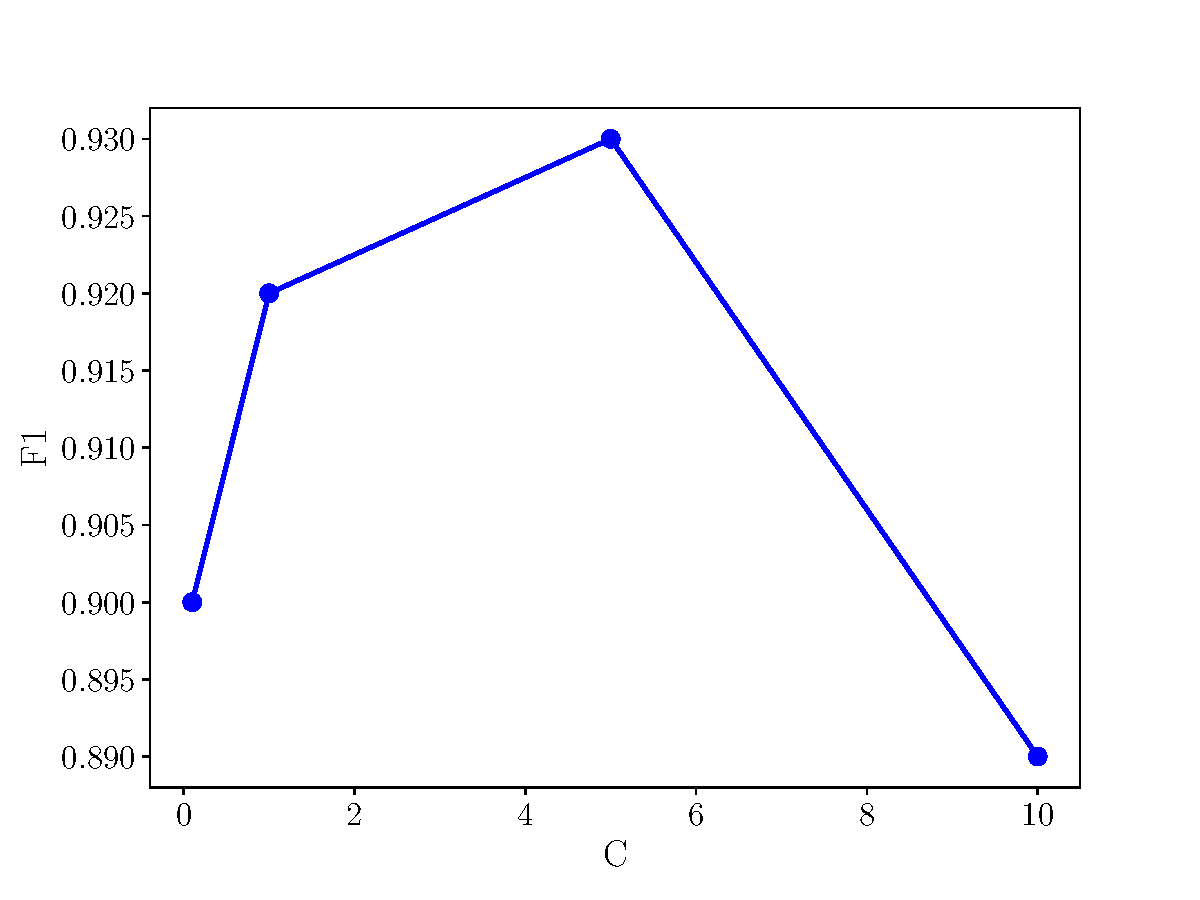
\includegraphics[width=3.5in]{../notebooks/results.pdf}
	\caption{A caption}
	\label{fig:a_label}
\end{figure}

\section{Discussion}

In this project, we concatenated the output of neural nets in pursuit of ideal recomendations. The exact accuracy is unclear, and further evaluation is required to determine if this approach is superior to simply focusing on one technique for recomendation.Through 

\section{Conclusion}
The evaluation of our recommendation system will rely on objective measurements derived from the system's performance on a held-out test dataset. We will use metrics such as precision, recall, F1 score, and Mean Average Precision (MAP) to quantify the system's accuracy in predicting user preferences based on their input and interaction history. Comparison with a baseline model, such as traditional collaborative filtering without real-time user input, will highlight improvements. We'll also utilize confusion matrices to analyze the model's performance in different recommendation scenarios, providing a detailed view of its strengths and areas for improvement. This method ensures an objective and comprehensive evaluation without the need for live deployment or user feedback.

\section{Division of Labor}
Lorem ipsum dolor sit amet, consectetur adipiscing elit, sed do eiusmod tempor incididunt ut labore et dolore magna aliqua. Ut enim ad minim veniam, quis nostrud exercitation ullamco laboris nisi ut aliquip ex ea commodo consequat. Duis aute irure dolor in reprehenderit in voluptate velit esse cillum dolore eu fugiat nulla pariatur. Excepteur sint occaecat cupidatat non proident, sunt in culpa qui officia deserunt mollit anim id est laborum.





\bibliography{references}
\bibliographystyle{acl_natbib}


\end{document}
